\documentclass[oneside,senior,etd]{BYUPhys}

\usepackage{cmap} % Для корректной кодировки в pdf
\usepackage[utf8]{inputenc}
\usepackage{rotating}

\usepackage[russian]{babel}
\usepackage{amsfonts} % Пакеты для математических символов и теорем
\usepackage{amstext}
\usepackage{amssymb}
\usepackage{amsthm}
\usepackage{graphicx} % Пакеты для вставки графики
%\usepackage{subfig}
\usepackage{color}
\usepackage[unicode]{hyperref}
\usepackage[nottoc]{tocbibind} % Для того, чтобы список литературы отображался в оглавлении
\usepackage{verbatim} % Для вставок заранее подготовленного текста в режиме as-is
\usepackage{listings}

\newcommand{\sectionbreak}{\clearpage} % Раздел с новой станицы

\usepackage{tikz}
\usepackage{pgfplots}
\usetikzlibrary{arrows,positioning}
\usepackage{adjustbox}

\usepackage{makecell}
\usepackage{booktabs}
\usepackage{boldline}

\usepackage{xcolor}
\usepackage{soul}
\usepackage{url}
\usepackage{multirow}
\usepackage{amsmath}

\usepackage{pifont}
\usepackage{indentfirst} % Делать отступ в начале первого параграфа

\usepackage{minted}

\usepackage[inline]{enumitem}
\usepackage{subcaption}

\renewcommand
\listingscaption{Листинг}

% Общие параметры листингов
\lstset{
  %frame=TB,
  showstringspaces=false,
  tabsize=4,
  basicstyle=\linespread{1.0}\tt\small, % делаем листинги компактнее
  breaklines=true,
  texcl=true, % русские буквы в комментах
  captionpos=b,
  aboveskip=\baselineskip,
  commentstyle=\tt
}

\newcommand{\todo}[1]{\textcolor{red}{#1}}

% DEBUG
% \usepackage{showframe}

\Faculty{Факультет вычислительной математики и кибернетики}
\Chair{Кафедра системного программирования}
\Course{Параллельные высокопроизводительные вычисления}
\Year{2024}
  \Date{7 Ноября}
  \City{Москва}
  \AuthorText{Автор:}
  \Author{Егоров Илья Георгиевич}
  \AuthorEng{Ilya Yegorov}
  \AcadGroup{527}

  \TitleTop{Многопоточная реализация операций с сеточными данными}
  % Раскомментируйте, если нужны еще строчки названия
  \TitleMiddle{на неструктурированной смешанной сетке,}
  \TitleBottom{решение системы линейных алгебраических уравнений}
  % Uncomment if you need English title
  % \TitleTopEng{Thesis theme, first line}
  % \TitleMiddleEng{Thesis theme, second line}
  % \TitleBottomEng{Thesis theme, third line}

\docname{ОТЧЁТ}                                      

%%%% DON'T change this. It is here because .sty does not support cyrillic cp properly %%%%
\TitlePageText{Титульная страница}
\University{Московский государственный университет имени М.В.Ломоносова}
\GrText{группа}
\ListingText{Листинг}
\AlgorithmText{Алгоритм}

% Set PDF title and author
\hypersetup{
  pdftitle={\PDFTitle},
  pdfauthor={\PDFAuthor}
}

\begin{document}
\fixmargins
 \makepreliminarypages

\oneandhalfspace

\pdfbookmark[section]{\contentsname}{toc}
\tableofcontents

\section{Описание задания и программной реализации}

\subsection{Постановка задачи}

Работа программы состоит из 4 этапов:
\begin{enumerate}
  \item \textbf{Generate}~--- генерация графа/портрета по тестовой сетке;
  \item \textbf{Fill}~--- заполнение матрицы по заданному портрету;
  \item \textbf{Solve}~--- решение СЛАУ с полученной матрицей;
  \item \textbf{Report}~--- проверка корректности программы и выдача измерений. 
\end{enumerate}

\subsubsection{Генерация портрета на основе тестовой сетки}

Будем иметь дело с двухмерной неструктурированной смешанной сеткой, состоящей из
треугольников и четырехугольников.  Решетка состоит из $N = N_x * N_y$ клеточек.
У каждой клетки есть позиция $(x, y)$, где $i$~--- номер строки в решетке,
$j$~--- номер столбца. Нумерация клеток в решетке построчно слева направо,
сверху вниз. Номер клеточки в единой общей нумерации: $I = i * N_x + j$. Далее
часть квадратных клеток делятся на треугольники следующим образом: $K_1$ и
$K_2$~--- количество идущих подряд треугольников и четырехугольников
соотвественно. На данном этапе нужно сгенерировать "топологию" связей ячеек:
построить графа, и по нему сгенерировать портрет матрицы смежности, дополнив
этот портрет главной диагональю, где вершины графа~--- элементы сетки (вариант
Б2).

\textbf{Входные данные:}
\begin{itemize}
  \item $N_x, N_y$~--- число клеток в решетке по вертикали и горизонтали;
  \item $K_1, K_2$~--- параметры для количества треугольных и четырехугольных
    элементов.
\end{itemize}

\textbf{Выходные данные:}
\begin{itemize}
  \item $N$~--- размер матрицы (число вершин в графе);
  \item $IA, JA$~--- портрет разреженной матрицы смежности графа, (в формате
    CSR). 
\end{itemize}

\subsubsection{Построение СЛАУ по заданному портрету матрицы}

\textbf{Входные данные:}
\begin{itemize}
  \item $N$~--- размер матрицы (число вершин в графе);
  \item $IA, JA$~--- портрет разреженной матрицы смежности графа, (в формате
    CSR). 
\end{itemize}

\textbf{Выходные данные:}
\begin{itemize}
  \item $A$~--- массив ненулевых коэффициентов матрицы (размера $IA[N]$);
  \item $b$~--- вектор правой части (размера $N$).
\end{itemize}

Правила заполнения:
\begin{itemize}
  \item $a_{ij} = \cos(i * j + i + j), i \neq j, j \in Col(i)$
  \item $a_{ii} = 1.234 \sum_{j, j \neq i} |a_{ij}|$
  \item $b_i = \sin(i)$
\end{itemize}

\subsubsection{Решение СЛАУ итерационным методом}

\textbf{Входные данные:}
\begin{itemize}
  \item $N$~--- размер матрицы (число вершин в графе);
  \item $IA, JA$~--- портрет разреженной матрицы смежности графа, (в формате
    CSR). 
  \item $A$~--- массив ненулевых коэффициентов матрицы (размера $IA[N]$);
  \item $b$~--- вектор правой части (размера $N$).
  \item $eps$~--- критерий остановки ($\epsilon$), которым определяется точность
    решения;
  \item $maxit$~--- максимальное число итераций.
\end{itemize}

\textbf{Выходные данные:}
\begin{itemize}
  \item $x$~--- вектор решения (размера $N$);
  \item $n$~--- количество выполненных итераций;
  \item $r$~--- L2 норма невязки (невязка – это вектор $r = Ax - b$).
\end{itemize}

Будем использовать такой алгоритм предобусловленного метода CG.

Для решателя понадобится несколько вычислительных функций для базовых операций:
\begin{itemize}
  \item Матрично-векторное произведение с разреженной матрицей (sparse
    matrix-vector);
  \item Скалярное произведение;
  \item Поэлементное сложение двух векторов с умножением одного из них на
    скаляр.
\end{itemize}

\subsubsection{Проверка корректности программы и выдача измерений}

На этом этапе нужно проверить, что невязка системы удовлетворяет заданной
точности, выдать значение фактической невязки, и распечатать табличку
таймирования, в которой указано, сколько времени в секундах затрачено на:
\begin{enumerate}
  \item Этап генерации;
  \item Этап заполнения;
  \item Этап решения СЛАУ;
  \item Каждую из трех кернел-функций, базовых алгебраических операций решателя
    СЛАУ.
\end{enumerate}

\subsection{Программная реализация}

Программа реализована на языке C++ (с++11/c++17).

На листинге~\ref{list:help} представлен интерфейс программы.
\begin{listing}[p]
  \caption{Интерфейс реализованной программы}
  \label{list:help}
\begin{minted}{bash}
Usage: ../solver Nx Ny K1 K2 Maxit Eps Tn Ll
Where:
Nx is positive int that represents grid hieght
Ny is positive int that represents grid width
K1 is positive int that represents square cells sequence length
K2 is positive int that represents triangular cells sequence length
Maxit is positive int that represents maximum iteration number
Eps is positive float that represents accuracy
Tn is tread numberLl is log level:
	<=0 - no logs
	>=1 - show time
	>=2 - show info
	>=3 - show arrays
\end{minted}
\end{listing}

Для хранения матриц векторов использовался стандартный \textit{std::vector}, для
возврата результата часто использовался \textit{std::pair} и \textit{std::tuple}
(удобно для c++17 и выше). Основные релизованные функции:
\begin{itemize}
  \item gen~--- функция генерации портрета матрицы;
  \item fill~--- функция построения СЛАУ по портрету матрицы;
  \item solve~--- функция-решатель СЛАУ;
  \item scalar~--- функция, вычисляющая скалярное произведение;
  \item sum\_vvc~--- функция, вычисляющая поэлементное сложение двух векторов с
    умножением одного из них на скаляр;
  \item mul\_mv~--- функция, вычисляющая матрично-векторное произведение с
    разреженной матрицей (sparse matrix-vector).
\end{itemize}

Более подробное описание функций можно найти в приложении~\ref{sec:appendix}.

\section{Исследование производительности}

\subsection{Характеристики вычислительной системы}

\noindent
Имя: ПВС «IBM Polus» \\
Пиковая производительность: 55.84 TFlop/s \\
Производительность (Linpack): 40.39 TFlop/s \\
Вычислительных узлов: 5 \\
На каждом узле: \\
Процессоры IBM Power 8: 2 \\
NVIDIA Tesla P100: 2 \\
Число процессорных ядер: 20 \\
Число потоков на ядро: 8 \\
Оперативная память: 256 Гбайт (1024 Гбайт узел 5) \\
Коммуникационная сеть: Infiniband / 100 Gb \\
Система хранения данных: GPFS \\
Операционная система: Linux Red Hat 7.5 

\subsection{Результаты измерений производительности}

Все измерения проводились со следующими параметрами:
\begin{itemize}
  \item $K_1 = 101$
  \item $K_2 = 57$
  \item $maxit = 1000$
  \item $eps = 0.0001$
\end{itemize}
Параметры $K_1$ и $K_2$ были выбраны взаимнопростыми друг с другом и с
размерностями сетки для большей хаотичности, выбор $maxit$ особо не на что не
влияет, так как при заданной точности $eps$ алгоритм сходится достаточно быстро
(при общем размере сетки порядка $9 * 10^9$ вершин алгоритм сходится всего за 25
итераций).

Используемые опции компиляции: \textit{-std=c++11 -O1 -fopenmp}
 
\subsubsection{Последовательная производительность}

Линейный линейный рост потребления памяти и времени работы в зависимости от
размера системы видны на на таб. \ref{tab:cons}, а также рис. \ref{fig:mem} и
рис. \ref{fig:time} соответственно.

\begin{table}[h]
  \centering
  \caption{Зависимость потребления памяти и времени работы от размера системы}
  \label{tab:cons}
  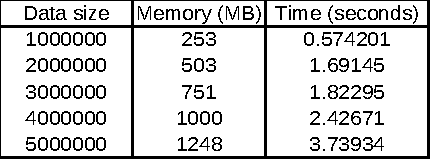
\includegraphics{images/consistent_performance.pdf}
\end{table}

\begin{figure}[h]
   \begin{minipage}{0.48\textwidth}
     \centering
     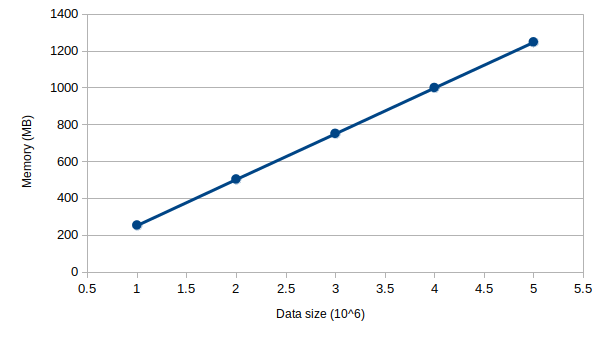
\includegraphics[width=\linewidth]{images/linear_mem.png}
     \caption{Зависимость потребления памяти от размера системы}
     \label{fig:mem}
   \end{minipage}\hfill
   \begin{minipage}{0.48\textwidth}
     \centering
     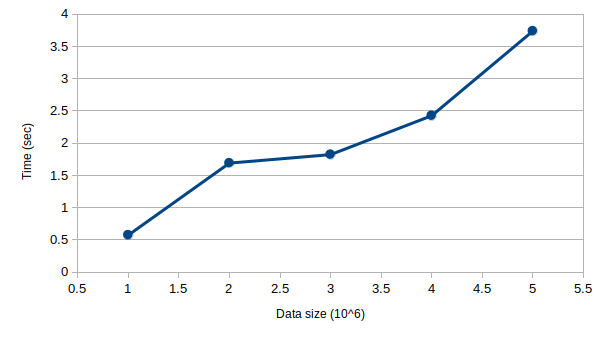
\includegraphics[width=\linewidth]{images/linear_time.png}
     \caption{Зависимость времени работы от размера системы}
     \label{fig:time}
   \end{minipage}
\end{figure}

На таб. \ref{tab:flops} и рис. \ref{fig:flops} показана зависимость достигаемой
  производительности от размера системы для всего алгоритма решателя.

\begin{table}[h]
  \centering
  \caption{Зависимость достигаемой производительности от размера системы}
  \label{tab:flops}
  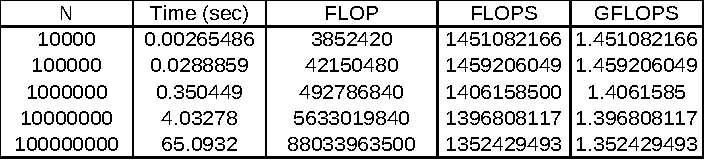
\includegraphics[width=\textwidth]{images/gflops.pdf}
\end{table}

\begin{figure}[h]
   \centering
   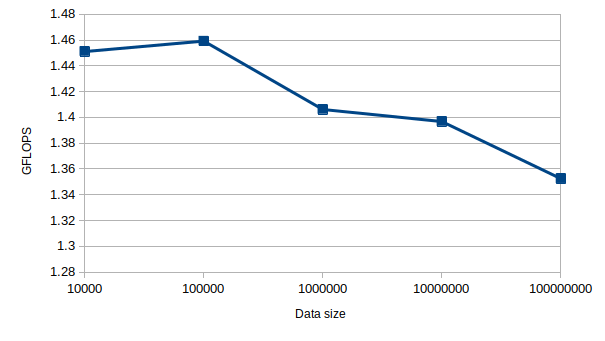
\includegraphics[width=\linewidth]{images/gflops.png}
   \caption{Зависимость достигаемой производительности от размера системы}
   \label{fig:flops}
\end{figure}

\subsubsection{Параллельное ускорение}

  На таб. \ref{tab:paral} и рис. \ref{fig:step} и \ref{fig:func} хорошо видно
наличие параллельного ускорения для разных этапов программы и основных функций
соответственно. Замеры производились с параметрами $N_x = 8000$ и $N_y = 8000$ и
привязкой к узлам \textit{polus-c3-ib} и \textit{polus-c4-ib} и ядрам.

\begin{table}[h]
  \centering
  \caption{Зависимость времени работы этапов программы и основных функций от
  числа параллельных  процессов}
  \label{tab:paral}
  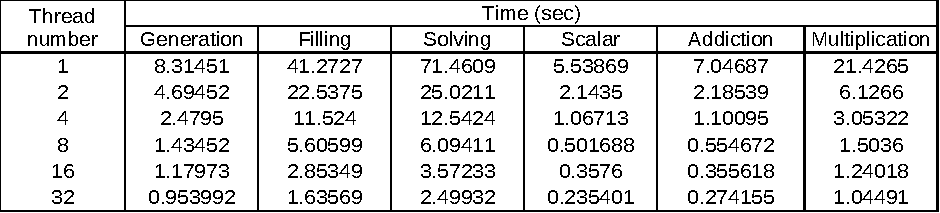
\includegraphics[width=\textwidth]{images/parallel_acceleration.pdf}
\end{table}

\begin{figure}[h]
   \begin{minipage}{0.48\textwidth}
     \centering
     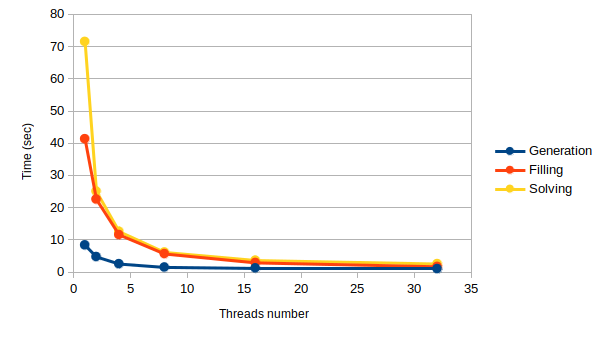
\includegraphics[width=\linewidth]{images/step_time.png}
     \caption{Зависимость времени работы этапов программы от числа параллельных
     процессов}
     \label{fig:step}
   \end{minipage}\hfill
   \begin{minipage}{0.48\textwidth}
     \centering
     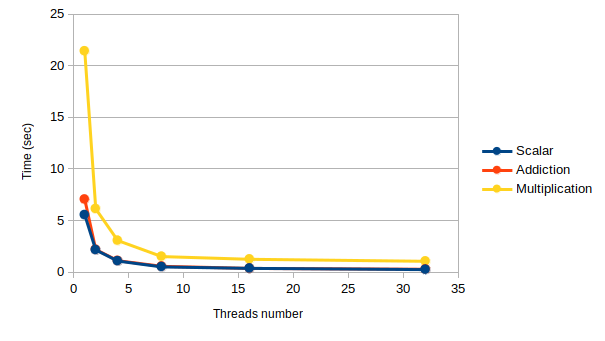
\includegraphics[width=\linewidth]{images/func_time.png}
     \caption{Зависимость времени работы основных функций от числа параллельных
     процессов}
     \label{fig:func}
   \end{minipage}
\end{figure}

\section{Анализ полученных результатов}

Рассчитаем $TBP$ (Theoretical Bounded Performance)~--- теоретически достижимую
производительность~--- и получаемый процент от неё для каждой из трех базовых
операций. $TBP$ рассчитывается по следующей формуле: $TBP = min(TPP, BW * AI)$,
где $TPP$ (Theoretical Peak Performance) – теоретическая пиковая
производительность, $BW$ (Bandwidth)~--- пропускная способность памяти, $AI$
(Arithmetic Intensity)~--- арифметическая интенсивность. Для Polus $TPP = 55.84
TFlop/s$, $BW = 153.6 GB/s$, а AI будет разной для разных функций. Для
скалярного произведения и сложения $AI$ будут фиксированными:
\begin{itemize}
  \item $AI_{scal} = \frac{2 * n}{2 * sizeof(float) * n} = \frac{1}{4}$
  \item $AI_{add} = \frac{2 * n}{3 * sizeof(float) * n} = \frac{1}{6}$
\end{itemize}
$AI$ для умножения матриц будет иметь более сложную зависимость. Путь $ia.size()
= n$, а $ja.size() = m$. Тогда $ia.size() = res.size() = v.size() = n$ и
$ja.size() = a.size() = m$, где все перечисленные вектора соответствую
аргументам функции \textit{mul\_mv} (подробнее в листинге \ref{list:mul}).
Отсюда имеем следующую формулу:
\begin{itemize}
  \item $AI_{mul} = \frac{2m}{sizeof(float)*(2m + 3n)} =\frac{m}{4m + 6n}$
\end{itemize}
$n$ и $m$ будут зависеть от количества вершин в графе, т.е. от каждого из
параметров $N_x$, $N_y$, $K_1$, $K_2$. Для значений параметров $N_x = 8000$,
$N_y = 8000$, $K_1 = 101$, $K_2 = 57$ получается следующий результат:

$n = 87088592$, $m = 389233773$, $AI_{mul} = \frac{389233773}{2079466644} \approx 0.187$

Получаем следующий результат:
\begin{itemize}
  \item $TBP_{scal} = 38.4 GFlops, \frac{TBP_{scal}}{TPP} \approx 0.067\%$
  \item $TBP_{add} \approx 25.6 GFlops, \frac{TBP_{add}}{TPP} \approx 0.045\%$
  \item $TBP_{mul} \approx 28,75 GFlops, \frac{TBP_{mul}}{TPP} \approx 0.05\%$
\end{itemize}

\appendix

\cleardoublepage \phantomsection
\section*{Приложение}\label{sec:appendix}
\addcontentsline{toc}{section}{Приложение}

В листингах~\ref{list:gen}, \ref{list:fill}, \ref{list:solve}, \ref{list:scal},
\ref{list:add} и \ref{list:mul} приведены прототипы и описания основных
реализованных функций.

\begin{listing}[h]
  \caption{Функция генерации портрета матрицы}
  \label{list:gen}
\begin{minted}{C}
/* Generate CSR portrait by grid params
 * # Arguments:
 * * nx - grid hieght
 * * ny - grid width 
 * * k1 - square cells sequence length
 * * k2 - triangular cells sequence length
 * * ll - log level
 * # Return values:
 * * ia - row CSR array
 * * ja - col CSR array
 * * t - time
 */
std::tuple<std::vector<size_t>, std::vector<size_t>, double>
gen(
    size_t nx,
    size_t ny,
    size_t k1,
    size_t k2,
    LogLevel ll
);
\end{minted}
\end{listing}

\begin{listing}[h]
  \caption{Функция построения СЛАУ по портрету матрицы}
  \label{list:fill}
\begin{minted}{C}
/* Fill val CSR array by given row/col arrays and right side array
 * # Arguments:
 * * ia - row CSR array
 * * ja - col CSR array
 * # Return values:
 * * a - val CSR array
 * * b - right side array
 * * t - time
 */
std::tuple<std::vector<float>, std::vector<float>, double>
fill(
    std::vector<size_t>& ia,
    std::vector<size_t>& ja
);
\end{minted}
\end{listing}

\begin{listing}[h]
  \caption{Функция-решатель СЛАУ}
  \label{list:solve}
\begin{minted}{C}
/* Solve Ax=b system
 * # Arguments:
 * * n - size
 * * ia - A row CSR array
 * * ja - A col CSR array
 * * a - A val CSR array
 * * b - right side array
 * * eps - accuracy
 * * maxit = maximum iteration number
 * * ll - log level
 * # Return values:
 * * x - solution
 * * k - iteration number
 * * r - residual
 * * t - operation time tuple
 */
std::tuple<
  std::vector<float>,
  size_t,
  std::vector<float>,
  std::tuple<double, double, double, double>
>
solve(
    size_t n,
    std::vector<size_t>& ia,
    std::vector<size_t>& ja,
    std::vector<float>& a,
    std::vector<float>& b,
    float eps,
    size_t maxit,
    LogLevel ll
);
\end{minted}
\end{listing}

\begin{listing}[h]
  \caption{Функция, вычисляющая скалярное произведение}
  \label{list:scal}
\begin{minted}{C}
/* Compute scalar product of two vectors with equal sizes
 * # Arguments:
 * * a - first vector
 * * b - second vector
 * * n - size
 * # Return value:
 * * scalar product value
 * * computing time
 */
std::pair<float, double>
scalar(
    std::vector<float>& a,
    std::vector<float>& b,
    size_t n
);
\end{minted}
\end{listing}

\begin{listing}[h]
  \caption{Функция, вычисляющая поэлементное сложение двух векторов с умножением
  одного из них на скаляр}
  \label{list:add}
\begin{minted}{C}
/* Store sum of two vectors with equal sizes (second with coef)
 * to preallocated vector
 * # Arguments:
 * * res - allocated result vector
 * * a - first vector
 * * b - second vector
 * * c - second vector coefficient
 * * n - size
 * # Return value:
 * * computing time
 */
double sum_vvc(
    std::vector<float>& res,
    std::vector<float>& a,
    std::vector<float>& b,
    float c,
    size_t n
);
\end{minted}
\end{listing}

\begin{listing}[h]
  \caption{Функция, вычисляющая матрично-векторное произведение с разреженной
  матрицей}
  \label{list:mul}
\begin{minted}{C}
/* Store multiply square CSR matrix by vector to preallocated vector
 * # Arguments:
 * * res - allocated result vector
 * * ia - row CSR array
 * * ja - col CSR array
 * * a - val CSR array
 * * v - vector
 * * n - size
 * # Return value:
 * * computing time
 */
double mul_mv(
    std::vector<float>& res,
    std::vector<size_t>& ia,
    std::vector<size_t>& ja,
    std::vector<float>& a,
    std::vector<float>& v,
    size_t n
)
\end{minted}
\end{listing}

\end{document}
